\chapter{Hamiltonian Monte Carlo}\label{ch:hmc}

The random walk Metropolis--Hastings algorithm explored in
\cref{ch:bayesian} generates proposals by perturbing the current state
with isotropic Gaussian noise. This strategy ignores the geometry of the
posterior: proposals are equally likely in every direction, regardless of
whether the posterior is steep or flat. Now that we have the ability to
differentiate through the forward map, we can exploit gradient information
to guide the sampler along the posterior surface. \emph{Hamiltonian Monte
Carlo} (HMC)~\cite{betancourt2018hamiltonian,neal2011mcmc} does precisely
this by borrowing the formalism of Hamiltonian dynamics to construct
proposals that are both distant from the current state and likely to be
accepted.

The physical intuition is as follows. We imagine the current position of
the Markov chain as a particle moving in the parameter space. At each
step, the particle is given a random kick (a momentum draw) and then
allowed to evolve under a Hamiltonian that couples its position to the
posterior. Because the dynamics conserve energy, the particle naturally
spends more time in regions of high posterior density and traces out
long-range, low-energy trajectories that would take a random walk many
steps to traverse.

\section{The Hamiltonian}\label{sec:hamiltonian}

Let $q \in \mathbb{R}^d$ denote the position (i.e.\ the parameter
vector~$\phi$; we use $q$ to follow the Hamiltonian mechanics convention)
and introduce an auxiliary momentum variable $p \in \mathbb{R}^d$. We
define the joint density of position and momentum through the canonical
distribution
\begin{equation}
  P(q, p) \propto \exp\!\big({-H(q, p)}\big),
  \label{eq:canonical-distribution}
\end{equation}
where $H(q, p)$ is the Hamiltonian. We decompose $H$ into a potential
energy~$U(q)$ and a kinetic energy~$K(p)$:
\begin{equation}
  H(q, p) = U(q) + K(p).
  \label{eq:hamiltonian-decomposition}
\end{equation}
This separation ensures that the joint density factorises as
$P(q, p) \propto \exp(-U(q))\,\exp(-K(p))$, so the position and momentum
are independent: marginalising over~$p$ recovers the target distribution
over~$q$ alone. We define the potential energy as the negative
log-posterior,
\begin{equation}
  U(q) = -\log p(q \mid \mathbf{y}) = -\ell(q) + \text{const},
  \label{eq:potential-energy}
\end{equation}
where the constant absorbs the normalising factor. Regions of high
posterior density correspond to low potential energy, so the particle
rolls into valleys at the posterior modes and must climb uphill to
escape. The kinetic energy is the quadratic form
\begin{equation}
  K(p) = \tfrac{1}{2}\, p^T M^{-1} p,
  \label{eq:kinetic-energy}
\end{equation}
where $M \in \mathbb{R}^{d \times d}$ is a symmetric positive-definite
\emph{mass matrix}. Under~\cref{eq:canonical-distribution} the momentum
is distributed as $p \sim \mathcal{N}(0, M)$. A well-chosen~$M$ that
approximates the posterior covariance preconditions the dynamics so that
the particle explores all directions at a similar rate.

\section{Leapfrog Integration and Metropolis
Correction}\label{sec:hmc-algorithm}

Hamilton's equations of motion for the
system~\cref{eq:hamiltonian-decomposition} are
\begin{equation}
  \frac{dq}{dt} = \frac{\partial H}{\partial p} = M^{-1}p,
  \qquad
  \frac{dp}{dt} = -\frac{\partial H}{\partial q} = -\nabla_q U(q).
  \label{eq:hamiltons-equations}
\end{equation}
The gradient $\nabla_q U(q) = -\nabla_q \ell(q)$ is computed via the
adjoint method described in \cref{ch:adjoint}. In practice these equations
are integrated numerically using the \emph{leapfrog} integrator, which is
symplectic and time-reversible. Given a step size~$\varepsilon$ and
$L$~integration steps, one leapfrog trajectory from $(q_0, p_0)$ proceeds
as:
\begin{equation}
  \begin{aligned}
    p_{i+1/2} &= p_i - \tfrac{\varepsilon}{2}\,\nabla_q U(q_i), \\
    q_{i+1}   &= q_i + \varepsilon\, M^{-1} p_{i+1/2}, \\
    p_{i+1}   &= p_{i+1/2}
    - \tfrac{\varepsilon}{2}\,\nabla_q U(q_{i+1}),
  \end{aligned}
  \label{eq:leapfrog}
\end{equation}
for $i = 0, 1, \ldots, L-1$. Each step requires one evaluation of
$\nabla_q U$, so a trajectory of $L$~steps costs $L$~gradient
evaluations, each involving a full forward and adjoint solve.

Because the leapfrog integrator introduces a discretisation error, the
Hamiltonian is not exactly conserved along the trajectory. To ensure
the chain targets the correct stationary distribution, a Metropolis
acceptance step is applied: the endpoint $(q^*, p^*)$ of the trajectory
is accepted with probability

\begin{equation}
  r = \min\!\big\{1,\;
  \exp\!\big(H(q, p) - H(q^*, p^*)\big)\big\}.
  \label{eq:hmc-acceptance}
\end{equation}

Since the integrator is symplectic, the energy error is typically small
and the acceptance rate is high even for proposals that are far from the
current state. The momentum is discarded after each accept/reject
decision; a fresh draw from $\mathcal{N}(0, M)$ at the start of each
iteration randomises the energy level and ensures the particle explores
the full posterior.

\section{The No-U-Turn Sampler}\label{sec:nuts}

The efficiency of HMC depends on the step size~$\varepsilon$ and
trajectory length~$L$. If $L$ is too small the sampler reverts to
near-random-walk behaviour; if $L$ is too large the trajectory doubles
back on itself, wasting gradient evaluations. The \emph{No-U-Turn
Sampler} (NUTS)~\cite{hoffman2014no} eliminates the need to specify~$L$
by doubling the trajectory in both directions until a U-turn criterion is
met. At each doubling the algorithm checks whether the endpoints of the
trajectory are moving apart; when they begin to converge the trajectory
is terminated and a sample is drawn uniformly from the valid states along
it. This adaptive scheme sets the trajectory length automatically at each
iteration, requiring only the step size~$\varepsilon$ and mass
matrix~$M$ to be specified.

\section{Parameter Transformations}\label{sec:transformations}

The leapfrog integrator applies a uniform step size~$\varepsilon$ in
every coordinate. If the parameters live on different scales or have
bounded support, the sampler performs poorly: it may step outside the
feasible region or waste steps on parameters whose natural scale is much
smaller than the step size. We address this by transforming the
Butler--Volmer parameters to an unconstrained space in which all
coordinates have comparable scale.

The transfer coefficient is constrained to the unit interval,
$\alpha \in (0,1)$; we apply the logit transform
\begin{equation}
  \tilde{\alpha} = \operatorname{logit}(\alpha)
  = \log\!\left(\frac{\alpha}{1 - \alpha}\right).
  \label{eq:logit-alpha}
\end{equation}
The dimensionless rate constant is constrained to be positive,
$K_0 > 0$; we apply the log transform
\begin{equation}
  \tilde{K}_0 = \log K_0.
  \label{eq:log-K0}
\end{equation}
The formal potential~$\theta_f$ is already unconstrained and requires no
transformation. The sampler operates in the transformed space
$\tilde{\phi} = (\tilde{\alpha},\, \tilde{K}_0,\, \theta_f)$, these
proposals are then transformed back into the dimensionless parameters
before being run through the solver. We tape these transformation to
ensure the correctness of the gradient updates.

\section{Inference Workflow}\label{sec:workflow}

We now describe the full inference pipeline used for the
electron-transfer reaction. The same workflow is applied to the
heterogeneous and adsorption reactions in
\cref{ch:heterogeneous,ch:adsorption}.

\paragraph{Step~1: Diverse initialisation.}
We draw $N_{\mathrm{init}}$ starting points in the transformed parameter
space using a Latin hypercube sample (LHS) to ensure broad coverage of
the prior support.

\paragraph{Step~2: Gradient-based optimisation.}
Each starting point is optimised toward the posterior mode using ADAM with
a fixed budget of forward-solve equivalents, as described in
\cref{sec:init-results}. The run achieving the highest log-posterior
density is selected as the initial state for both samplers.

% TODO: Window adaption reference (stan?)

\paragraph{Step~3: Window adaptation.}
Starting from the optimised point, a NUTS warm-up phase of
$N_{\mathrm{adapt}}$~iterations is run. During this phase the step
size~$\varepsilon$ is tuned via dual averaging~\cite{hoffman2014no} and
the mass matrix~$M$ is estimated from the sample covariance of the warm-up
draws. For RWMH, the same warm-up covariance is used to set the proposal
covariance~$\Sigma$, scaled to achieve the $23\%$ acceptance rate
heuristic~\cite{gelman1997weak}.

\paragraph{Step~4: Sampling.}
Both NUTS and RWMH are run from the same initial state with the tuned
hyperparameters. To ensure a fair comparison the two samplers are given
equal computational budgets measured in forward-solve equivalents. Since
each NUTS iteration requires $L$~leapfrog steps (each costing one forward
and one adjoint solve) and each RWMH iteration requires one forward
solve, we allocate more RWMH iterations to match the total cost.

\section{Results}\label{sec:hmc-results}

\subsection{Posterior Distributions}

\Cref{fig:electron-posteriors} overlays the marginal posterior
distributions obtained by NUTS and RWMH for the electron-transfer
reaction. Both samplers recover the true parameter values, with the
marginals concentrating around the dashed lines at
$\phi^* = (0.6,\, 10.0,\, 0.5)$. The two sets of marginals are in close
agreement, confirming that both chains have converged to the same
target distribution. We also note that width of the distributions are
far tighter than what was observed in the previous chapter, which
shows that the optimisation step has removed the tail artifacts observed before.

We too run sampling for $\phi^* = (0.6,\,
500.0,\, 0.5)$ which is in the reversible reigime and as established,
this makes it harder to distinguish between parameters. This is
reflected in the sampling, as we see wider distributions over the
posterior space, while still having the distributions centered at the
true value which is exactly what we would like in this Bayesian setting.

\begin{figure}[ht]
  \begin{center}
    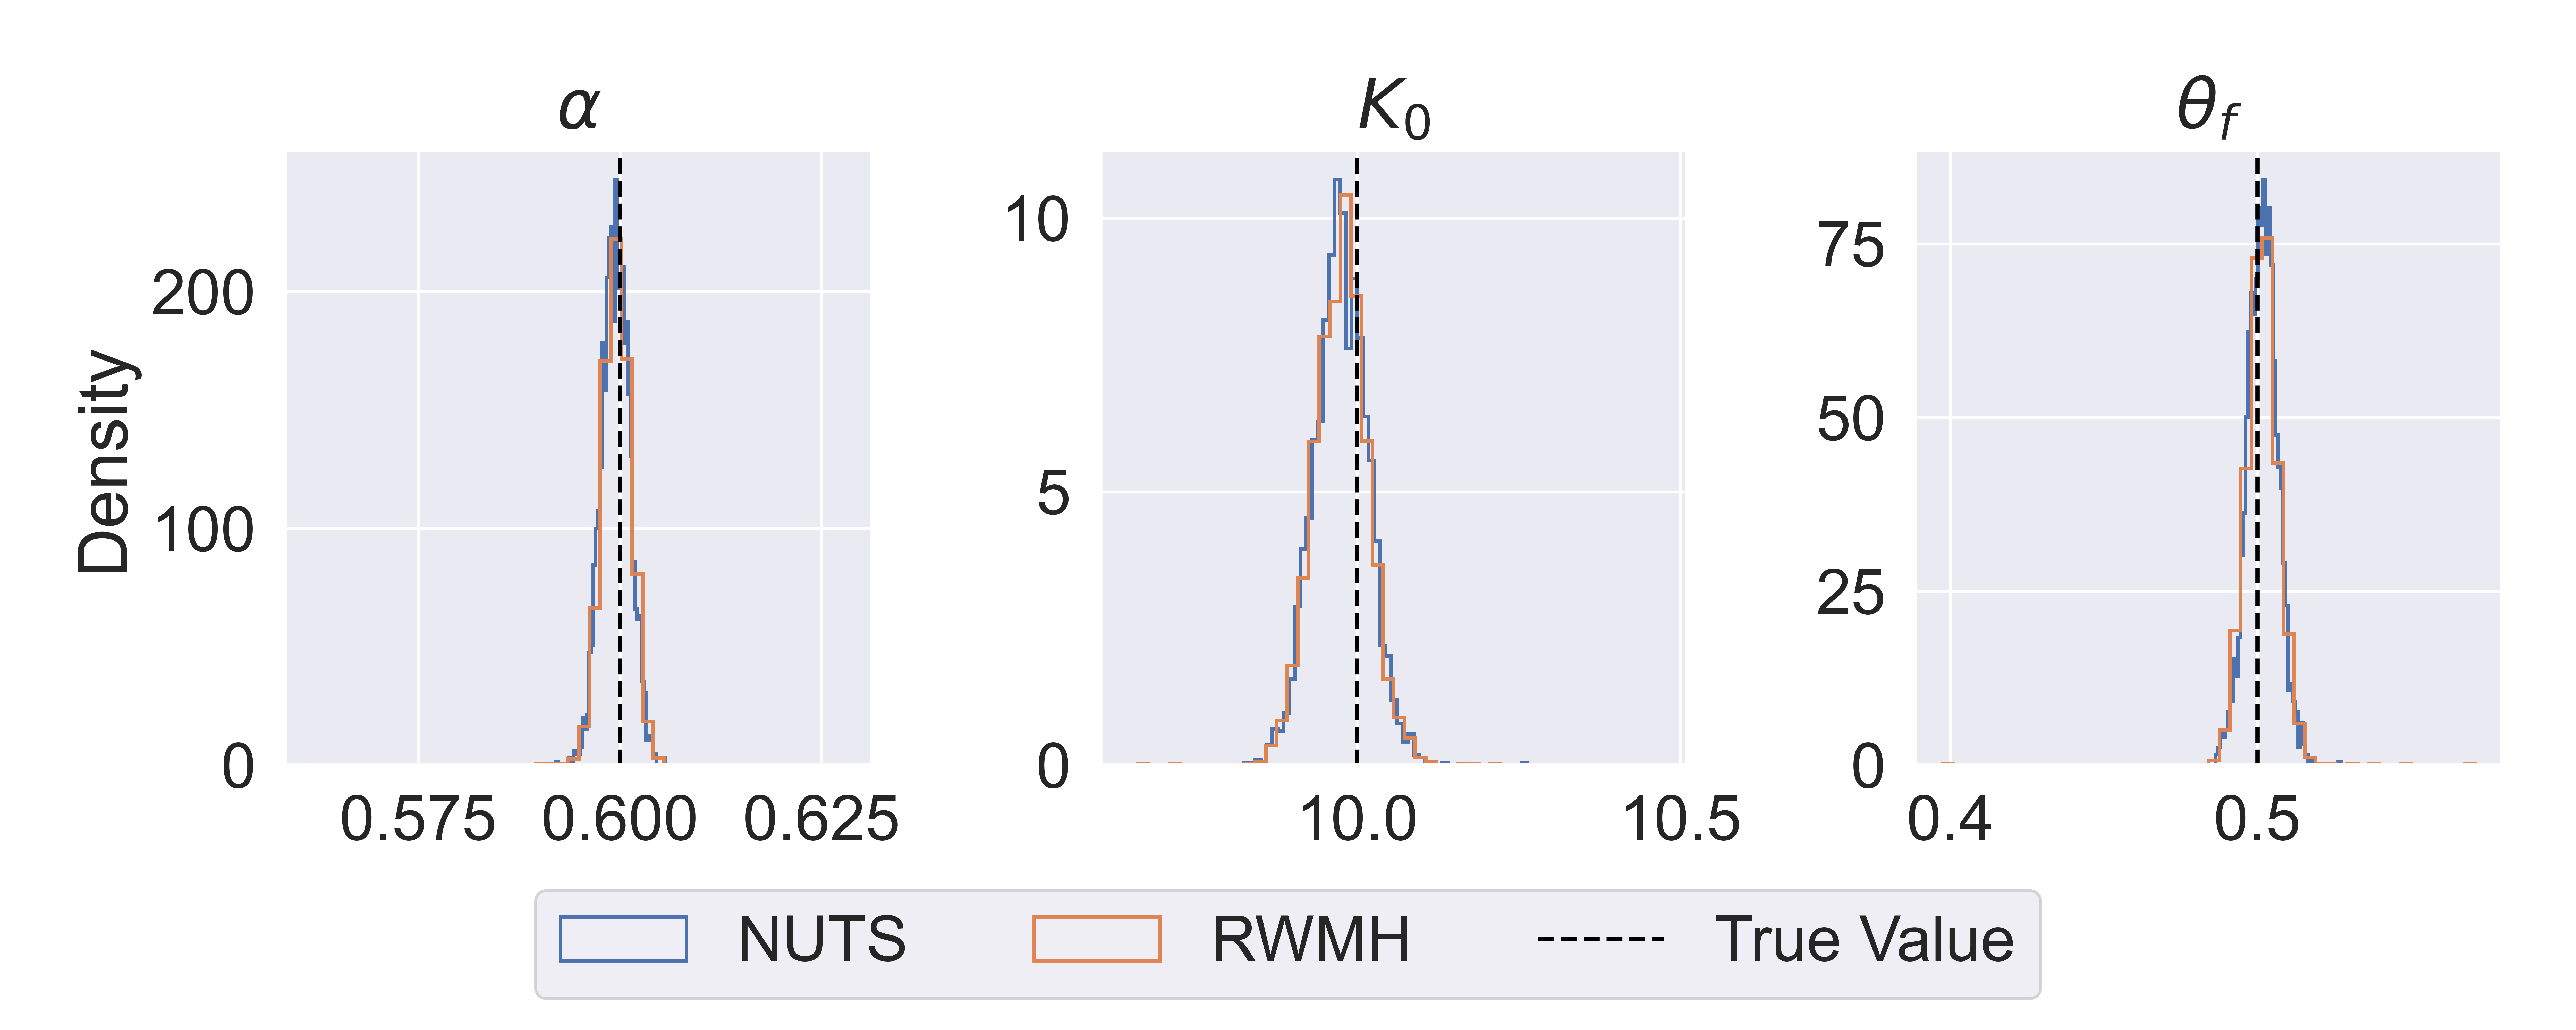
\includegraphics[width=0.95\textwidth]{figures/6-hmc-hist.png}
  \end{center}
  \caption[Marginal posteriors from NUTS and RWMH for the
  electron-transfer reaction]{Marginal posterior distributions for the
    three Butler--Volmer parameters obtained by NUTS (blue) and RWMH
    (orange) under equal computational budgets. Dashed lines indicate
    the true parameter values. Both samplers recover the correct
  posterior.}
  \label{fig:electron-posteriors}
\end{figure}

\begin{figure}[ht]
  \begin{center}
    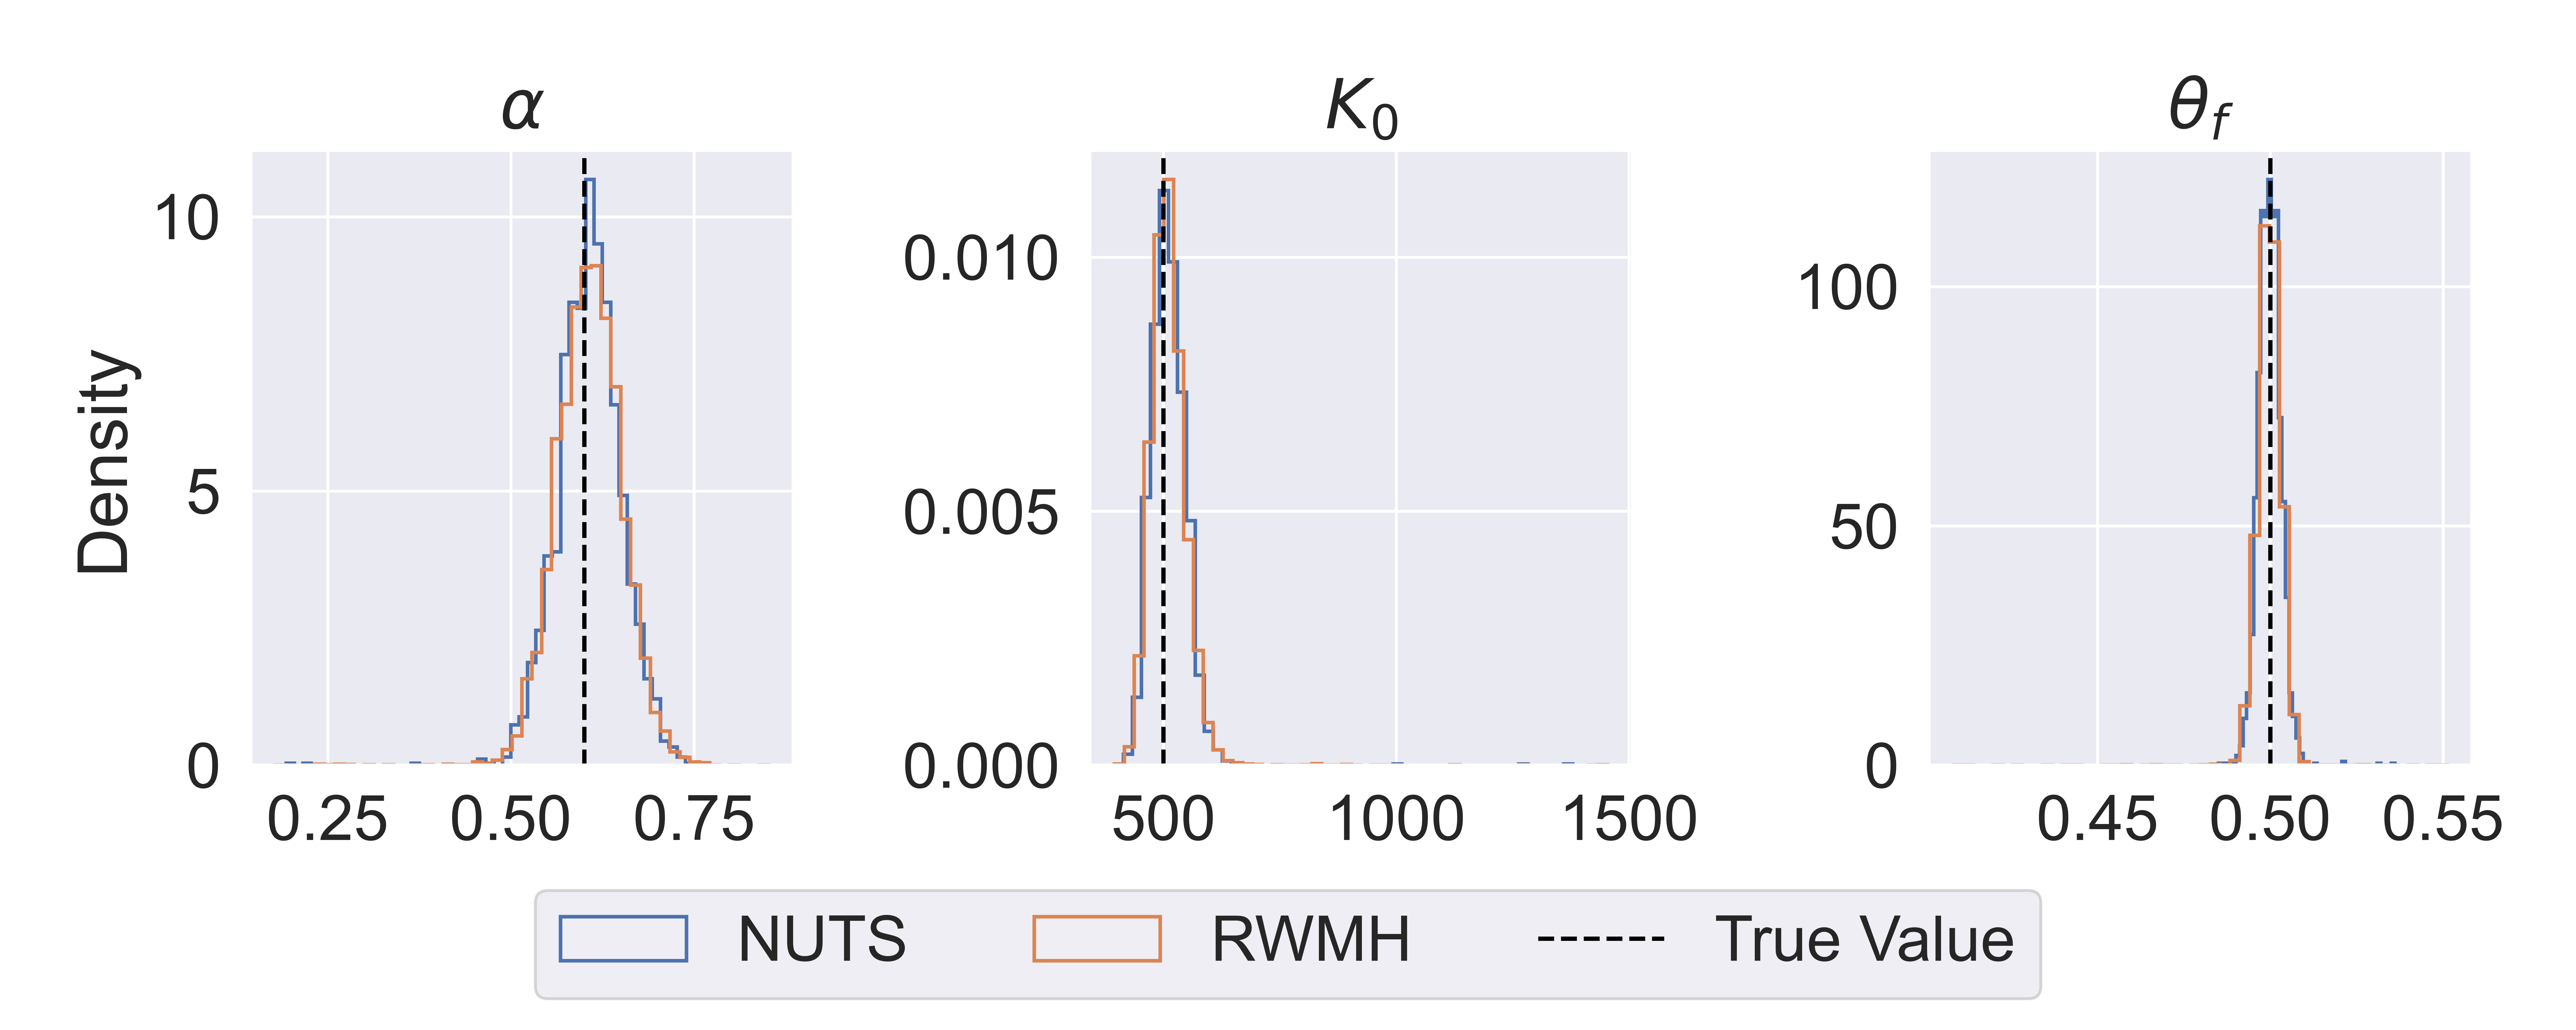
\includegraphics[width=0.95\textwidth]{figures/6-hmc-hist-rev.png}
  \end{center}
  \caption[Marginal posteriors from NUTS and RWMH for the
  electron-transfer reaction in the reversible regime]{Marginal
    posterior distributions for the
    three Butler--Volmer parameters obtained by NUTS (blue) and RWMH
    (orange) under equal computational budgets in the reversible
  regime. Dashed lines indicate the true parameter values.}
  \label{fig:electron-posteriors-rev}
\end{figure}

\Cref{fig:electron-current-fit} shows the simulated voltammogram
evaluated at the posterior mean from the NUTS chain against the true
parameter current. The close agreement confirms that the inferred
parameters reproduce the observed current response.

\begin{figure}[ht]
  \begin{center}
    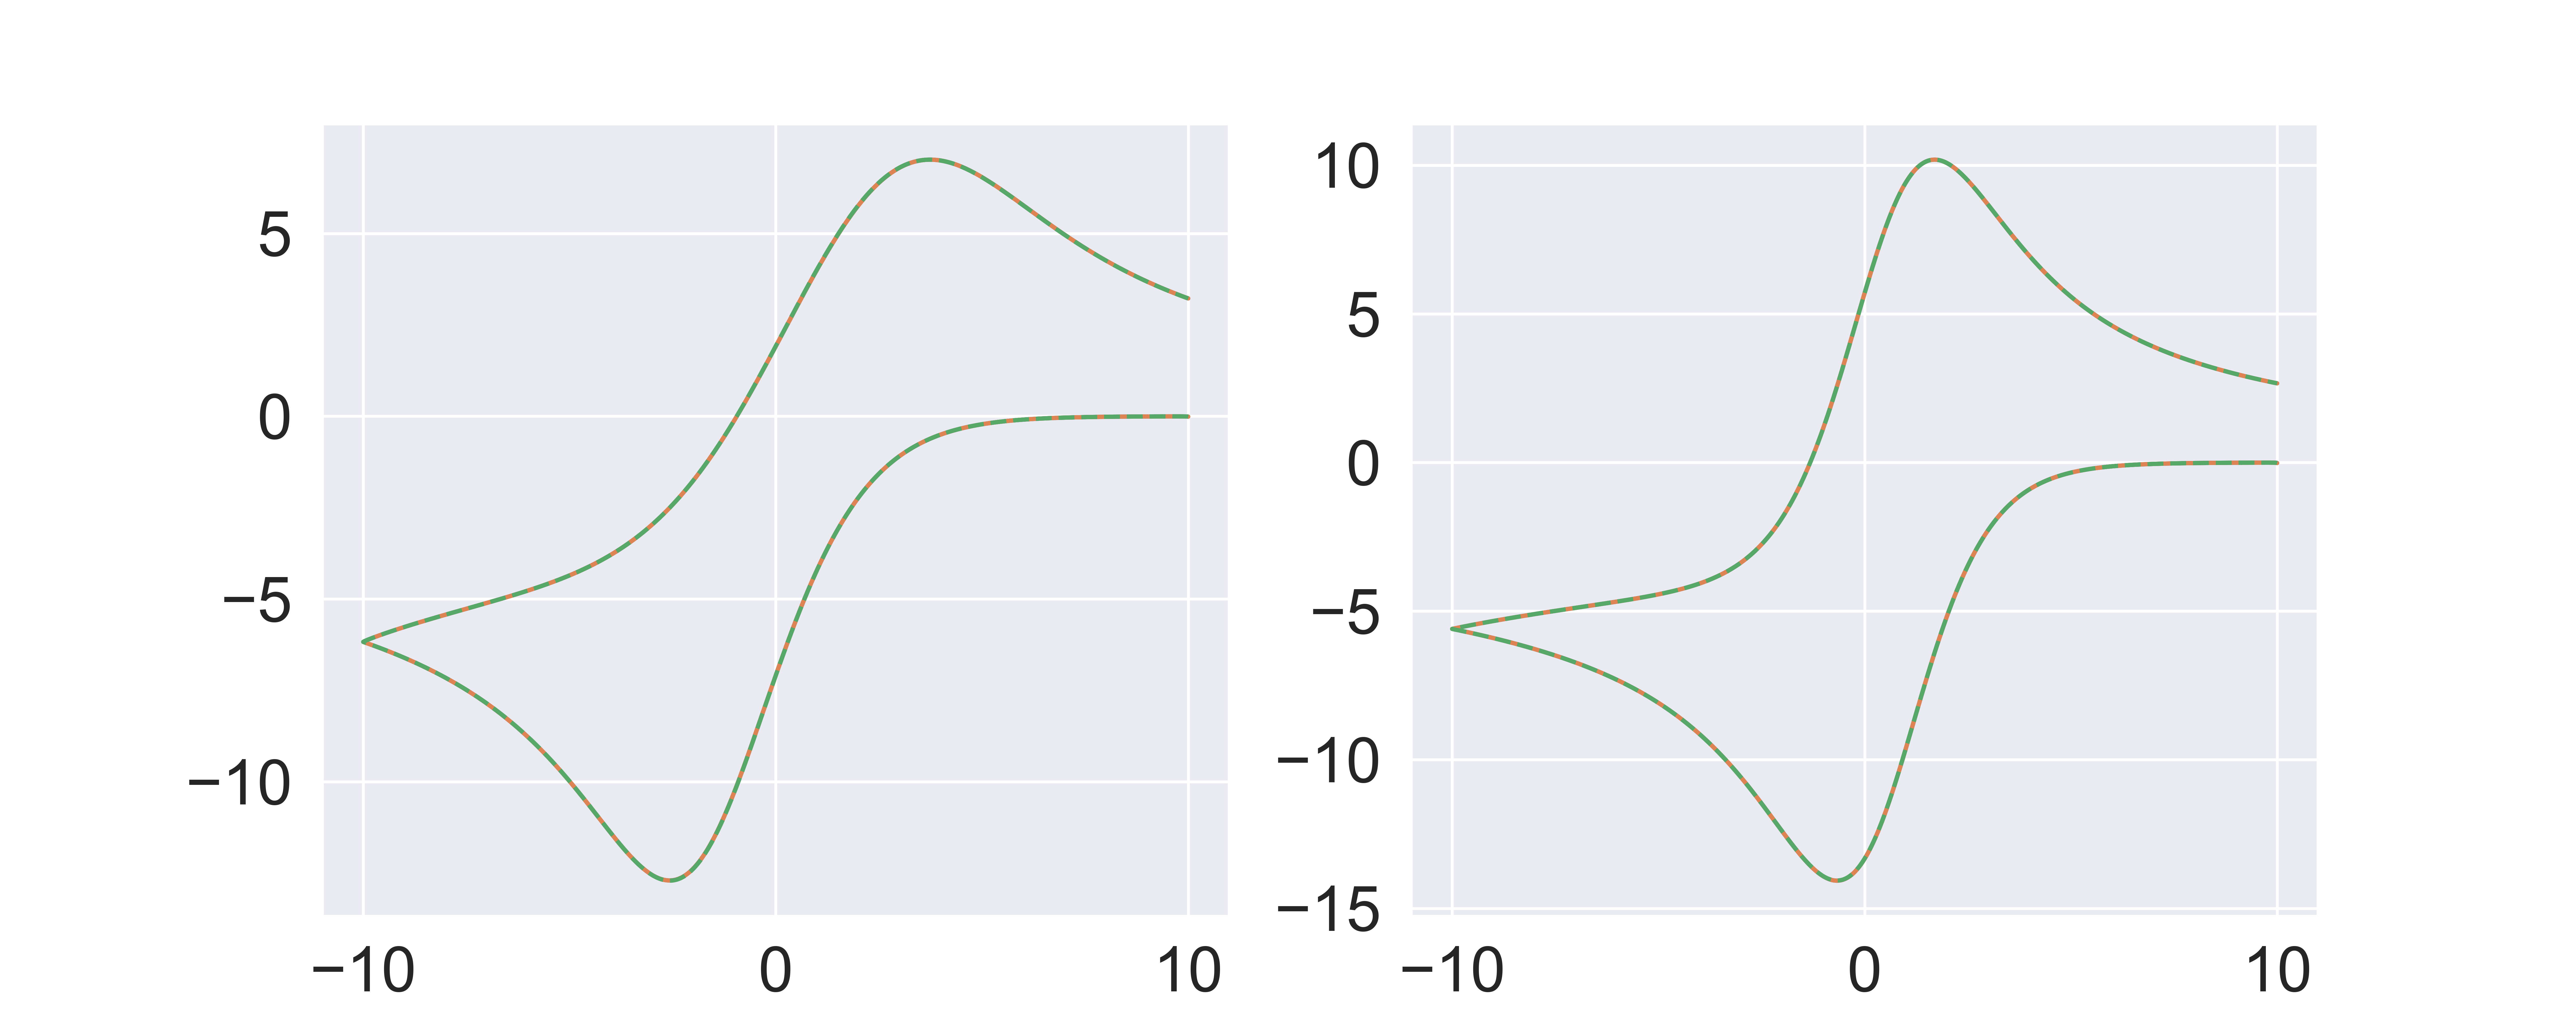
\includegraphics[width=0.7\textwidth]{figures/6-current-fit.png}
  \end{center}
  \caption[Posterior-mean current fit for the electron-transfer
  reaction]{Simulated voltammogram evaluated at the NUTS posterior
    mean, against the underlying true parameter voltammagrams. Left:
    Quasi-reversible reigime. Right: Reversible Reigime. The
    close agreement confirms that the inferred parameters reproduce the
  observed current.}
  \label{fig:electron-current-fit}
\end{figure}

\subsection{Effective Sample Size}

Any MCMC sampler produces serially correlated samples, so successive
draws carry less information than independent ones. The \emph{effective
sample size} (ESS)~\cite{gelman2013bayesian,geyer2011introduction}
quantifies the number of independent draws equivalent to the correlated
chain:
\begin{equation}
  \mathrm{ESS} = \frac{T}{1 + 2\sum_{k=1}^{\infty} \rho_k},
  \label{eq:ess}
\end{equation}
where $T$ is the total number of samples and $\rho_k$ is the
autocorrelation at lag~$k$.

\Cref{fig:electron-ess} compares the growth of ESS over the sampling
duration for NUTS and RWMH. The comparison is made on a normalised time
axis so that the two algorithms are compared at equal computational cost.
NUTS accumulates effective samples at a higher rate across all three
parameters. The advantage is most pronounced for~$K_0$, where NUTS
achieves roughly three times the ESS of RWMH at the end of the sampling
budget. \Cref{tab:electron-ess} reports the final ESS values for each
parameter.

\begin{table}[ht]
  \centering
  \begin{tabular}{lccc}
    \hline
    & $\alpha$ & $K_0$ & $\theta_f$ \\
    \hline
    NUTS & 2132.7 & 2986.7 & 2335.5 \\
    RWMH & 657.0 & 1634.0 & 761.0 \\
    \hline
  \end{tabular}
  \caption[Final ESS values for the electron-transfer reaction]{Effective
  sample size for each parameter at equal computational budget.}
  \label{tab:electron-ess}
\end{table}

\begin{figure}[ht]
  \begin{center}
    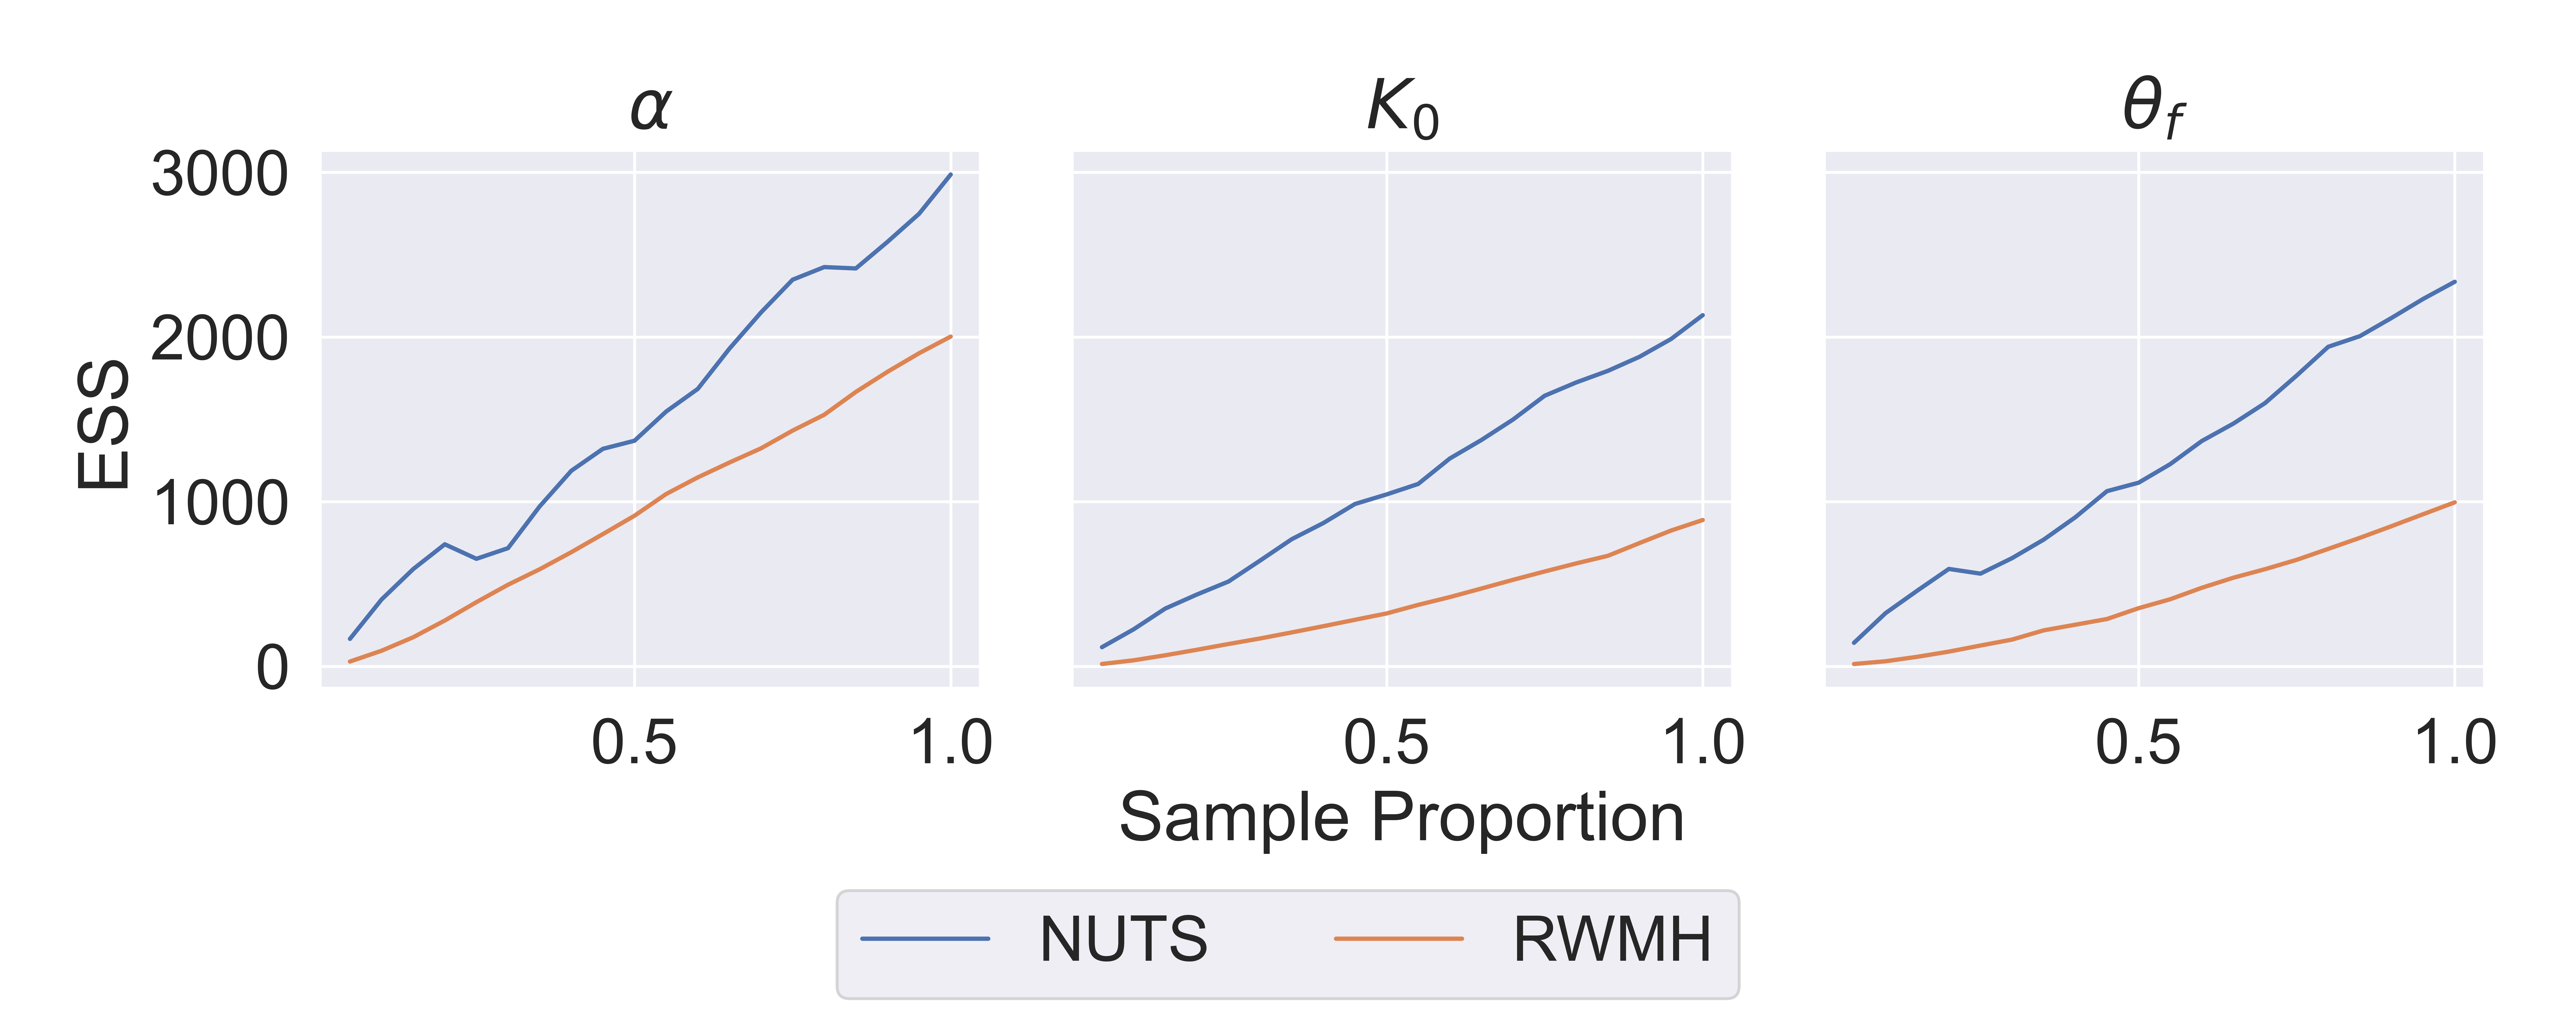
\includegraphics[width=0.95\textwidth]{figures/6-ess.png}
  \end{center}
  \caption[ESS comparison for NUTS and RWMH]{Effective sample size as a
    function of normalised computational time for NUTS (blue) and RWMH
    (orange), for each of the three Butler--Volmer parameters. The
    horizontal axis is normalised so that the two algorithms are compared
    at equal computational cost. NUTS achieves a higher ESS across all
  parameters, with the largest gain for~$K_0$.}
  \label{fig:electron-ess}
\end{figure}

With the inference framework now validated on the three-parameter
electron-transfer reaction, we apply it to reactions of increasing
complexity in the following chapters.
